% !TEX root = ../../../main.tex
% 来源：中学数学实验教材·第二册（几何）
% 章节：轨迹与作图 / 作图
% 原始文件：5.tex，行 686-701
% 类型：tikz
% ---
    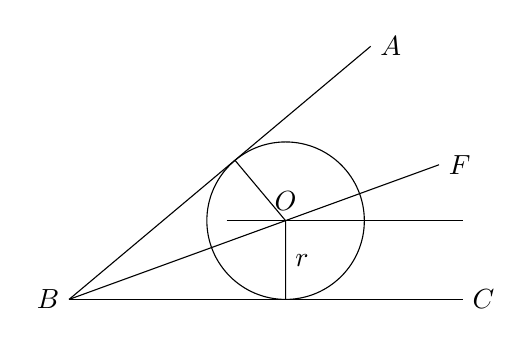
\begin{tikzpicture}[>=latex, scale=1]
\foreach \x/\xtext in {0/C,20/F,40/A}
{
    \draw(0,0)--(\x:5)node[right]{$\xtext$};
}
\draw(2,1)--(5,1);
\draw(2.75,1) circle(1);
\draw(2.75,0)--node[right]{$r$}(2.75,1)node[above]{$O$}--(40:2.75);
\node at (0,0) [left]{$B$};
\tkzDefPoint(40:2.75){D}
\tkzDefPoint(0:2.75){E}
\tkzDefPoint(2.75,1){O}\tkzDefPoint(0,0){B}
\tkzMarkRightAngles[size=.1](B,D,O B,E,O)


    \end{tikzpicture}
